\documentclass[11pt, oneside, titlepage]{article}
\usepackage{fancyhdr}
\usepackage{graphicx}
\usepackage{imakeidx}
\usepackage{makeidx}
\usepackage{mathtools}
\usepackage[spanish]{babel}
\usepackage{graphicx}
\usepackage{dsfont}
 
\title{\textbf{Álgebra lineal}\\ Universidad Católica de Santa Teresa de Jesús, Ávila}
\author{Francisco Javier Balón Aguilar}
\date{Febrero 2019}

\usepackage{amsmath}
\begin{document}
\maketitle
% Índice de contenidos
\tableofcontents
\newpage

\section{Conceptos previos}
\subsection{Álgebra de conjuntos}
Un conjunto es una colección de elementos con características similares considerada en sí misma como un objeto. Podemos hacer el símil con los \emph{arrays} o listas de elementos en los diferentes lenguajes de programación. Así, el conjunto X es un objeto que mantiene una serie de elementos, por ejemplo:
\[
X=\{0, 1, 2, 3, 4\}
\]

\[
Y=\{1, 2, 3\}
\]

Entonces:
\begin{enumerate}
\item Si $x = 0;\ x \in X;\ x \notin Y$; $x$ es un elemento de $X$ y no de $Y$. 
\item $X \neq Y$; $X$ no es igual que $Y$.
\item $Y \subseteq X$; todo elemento de $Y$ está en $X$; $Y$ es un subconjunto de $X$.
\end{enumerate}

Podemos realizar \textbf{operaciones con conjuntos}, que englobarían el tratamiento y las propiedades básicas de estas; siendo estas las siguientes:
\begin{enumerate}
\item \emph{Intersección.}

<<Dados dos conjuntos su intersección es el conjunto de elementos que están a la vez en los dos.>>

Entonces, dados los conjuntos $X=\{0,1,2,3\}$ e $Y=\{2,3,4,5\}$; 

$X \cap Y = \{2,3\}$, X intersección Y es \{2,3\}.

Dos conjuntos son \textbf{disjuntos} si su intersección es vacía; ($A \cap B = \emptyset$).
\item \emph{Unión.}

<<Dados dos conjuntos su unión es el conjunto de todos los elementos que están en alguno de ellos.>>

Entonces, dados los conjuntos $X=\{1,2,3\}$ e $Y=\{3,4,5\}$; 

$X \cup Y = \{1,2,3,4,5\}$; $X$ unión $Y$ es \{1,2,3,4,5\}.
\item \emph{Complementariedad.}

<<La complementariedad o complemento de un conjunto respecto a otro, es el conjunto de elementos del primero que no están en el segundo.>> ($X \backslash Y = \{x \in X : X \notin Y\}$).

Entonces, dados los conjuntos $X=\{0,1,2,3\}$ e $Y=\{1,3,5\}$;

$X \backslash Y = \{0,2\}$; el complemento de $X$ respecto a $Y$ es $\{0,2\}$.
\item \emph{Producto cartesiano.}

<<Dados dos conjuntos, su producto cartesiano es el conjunto de pares formados por un elemento del primero y un elemento del segundo.>> ($X \times Y = \{(x,y) : x \in X, y \in Y\}$).

Entonces, dados los conjuntos $X=\{0,1,2,3\}$ e $Y=\{4,5\}$;

El producto cartesiano de $X$ e $Y$ es (0,4)(0,5)(1,4)(1,5)(2,4)(2,5)(3,4)(3,5).
\end{enumerate}
 
\subsection{El número real}
El conjunto de números reales ($\mathds{R}$) que incluye tanto a números racionales (positivos, negativos y cero; $-\infty,-1,0,+1,+\infty$) y los números irracionales. Con este conjunto de números podemos definir operaciones y orden propio:

<<Los números reales forman un conjunto ($\mathds{R}$) dotado de dos operaciones: suma y producto.>>

Podemos establecer una \textbf{relación de orden} entre números reales ($\mathds{R}$):

Dados los números reales $x$ e $y$;

Entonces, si $x$ es mayor que $y$; $x > y$

Entonces, si $x$ es menor que $y$; $x < y$

Entonces, si $x$ es mayor o igual que $y$; $x \geq y$

Entonces, si $x$ es menor o igual que $y$; $x \leq y$

El \textbf{módulo} de un número real, denotado $|x|$ es un número real positivo que coincide con $x$, sea cual sea su signo. Así, $|5| = 5$ y $|-1| = 1$.

Existen dos clases de \textbf{intervalos}, en este caso refiriéndonos concretamente a los números reales:
\begin{enumerate}
\item \emph{Intervalos cerrados} [i].
\item \emph{Intervalos abiertos} (i).
\end{enumerate}
Estos intervalos se pueden combinar, siendo (1,2,3] un intervalo de inicio abierto y fin cerrado; siendo 1 y 2.
\subsection{Aplicaciones entre conjuntos}
<<Dados dos conjuntos, una aplicación entre ellos es una correspondencia que cada elemento de algún subconjunto del primero le asigna exactamente un elemento del segundo.>>

En resumen, una aplicación es una función con entrada y salida de información. Así como en programación encontramos funciones:
\[
def\ funcion(i):
	return\ i+1
\]
Así, una función o aplicación matemática sería:
\[
f(x)=x+1
\]
Dando como resultado el conjunto $Y$ a partir del conjunto $X = \{0,1,2\}$:
\[
f(0) = 1
\]
\[
f(1) = 2
\]
\[
f(\{0, 1, 2\}) = \{1, 2, 3\}
\]

La aplicación $g$ es la que asocia a cada número real con su módulo. Así, $g(x)=|x|$.

\subsubsection{Aplicaciones \emph{inyectivas}, \emph{sobreyectivas} y \emph{biyectivas}}
\begin{enumerate}
\item \emph{Aplicación inyectiva}. <<Una aplicación entre conjuntos es inyectiva si puntos distintos del dominio tienen imágenes distintas.>>
\begin{figure}[htp]
\centering
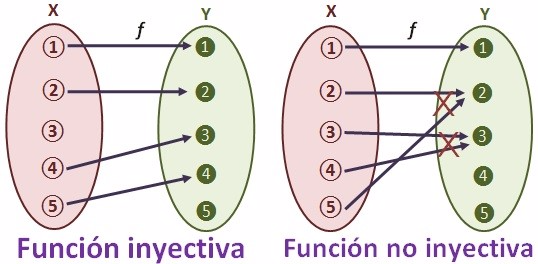
\includegraphics[width=0.9\textwidth]{recursos/finyectiva.png}
\caption{Gráfica de función inyectiva}
\label{}
\end{figure}

Así, en una función inyectiva no puede ocurrir que $f(x) = f(y)$, a no ser claro, que $x = y$.
\item \emph{Aplicación sobreyectiva}. <<Una aplicación es sobreyectiva si todos los puntos del conjunto llegada son alcanzados por algún punto del dominio.>>
\begin{figure}[htp]
\centering
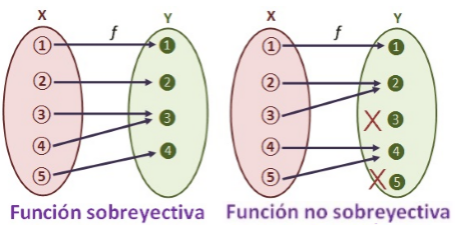
\includegraphics[width=0.9\textwidth]{recursos/fsobreyectiva.png}
\caption{Gráfica de función sobreyectiva}
\label{}
\end{figure}

Así, una función es sobreyectiva si todo elemento del conjunto final $Y$ tiene al menos un elemento del conjunto inicial $X$ al que le corresponde.
\item \emph{Aplicación biyectiva}. <<Una aplicación entre conjuntos es biyectiva si es a la vez inyectiva y sobreyectiva.>>
\begin{figure}[htp]
\centering
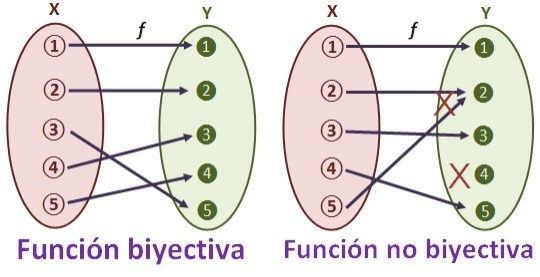
\includegraphics[width=0.9\textwidth]{recursos/fbiyectiva.png}
\caption{Gráfica de función biyectiva}
\label{}
\end{figure}
\end{enumerate}

\section{Espacios vectoriales}
Llamamos \emph{espacio vectorial} (sobre $\mathds{R}$) a un espacio $V$ equipado de dos operaciones:

\begin{enumerate}
\item \emph{Operación interna}. Verificando las siguientes propiedades:
\begin{enumerate}
\item \emph{Asociativa}. \[u+(v+w)=(u+v)+w\]
\item \emph{Conmutativa}. \[u+v=v+u\]
\item \emph{Existencia de elemento neutro} (existe 0). \[u+0=0+u=u\]
\item \emph{Existencia de elemento inverso}. \[u+(-u)=(-u)+u=0\]
\end{enumerate}
\item \emph{Operación externa} por elementos de $\mathds{R}$. Verificando las siguientes propiedades:
\begin{enumerate}
\item Siendo $a$ y $b$ escalares: \[a(a+v)=au+av\]
\item \[(a+b)u=au+bu\]
\item \[1u = u\]
\item \[a(bu)=(ab)u\]
\end{enumerate}
\end{enumerate}

Definimos $\mathds{R}^n$ como el conjunto de n-uplas de elementos de R:
\[\mathds{R}^n=\{(x_1...x_n)\} : x \in \mathds{R}\]
El producto cartesiano de $n$ copias del cuerpo de los números reales, $\mathds{R}^n$, \emph{\textbf{tiene una estructura natural de espacio vectorial real}}.

\subsection{Subespacios y dependencia lineal}
Sea $V$ un espacio vectorial. Un subespacio vectorial de $V$ es un subconjunto ($L$) de $V$. De modo que las operaciones de $V$ inducen operaciones de $L$ que le dotan de estructura de espacio vectorial.

Siendo $V$ un espacio vectorial y $v_1, v_2, v_3 ... \in V$. Se dice que $v$ es \emph{linealmente dependiente} de $v_1, v_2 ...$ si existen números reales $a_1, a_2...$ tales que:

\[
v=a_1 v_1+a_2v_2...
\]

\section{Aplicaciones lineales y matrices}
\subsection{Aplicación lineal}
Una aplicación lineal es una aplicación entre espacios vectoriales que respeta la suma de vectores y el producto por escalares. Hay que pensar aplicación como función.

Una aplicación $f : V \rightarrow W$ es una aplicación lineal si, y sólo si, para todos $u,v \in V$ y todos $a,b \in \mathds{R}$ se tiene que:
\[
f(au+bv)=af(u)+bf(v)
\]

\subsection{Matrices}
Sean $n,m$ enteros positivos. Una matriz $n \times m$ con entradas reales es una tabla de tamaño n x m. Tipos de matrices $A \in M_{nm}$:

\begin{enumerate}
\item \emph{Cuadrada}. $n=m$.
$\begin{pmatrix}
	a_{11} & a_{12} & a_{13}\\
	a_{21} & a_{22} & a_{23}\\
	a_{31} & a_{32} & a_{33}\\
\end{pmatrix}$
\item \emph{Triangular superior}. $a_{ij}=0$ para todo $i,j$ con $i > j$.
$\begin{pmatrix}
	a_{11} & a_{12} & a_{13}\\
	0 & a_{22} & a_{23}\\
	0 & 0 & a_{33}\\
\end{pmatrix}$
\item \emph{Triangular inferior}. $a_{ij}=0$ para todo $i,j$ con $i < j$.
$\begin{pmatrix}
	a_{11} & 0 & 0\\
	a_{21} & a_{22} & 0\\
	a_{31} & a_{32} & a_{33}\\
\end{pmatrix}$
\item \emph{Diagonal}. $a_{ij} = 0$ para todo $i,j$ con $i \neq j$.
$\begin{pmatrix}
	a_{11} & 0 & 0\\
	0 & a_{22} & 0\\
	0 & 0 & a_{33}\\
\end{pmatrix}$
\item \emph{Matriz identidad de orden $n$}. Matriz cuadrada $n \times n$, diagonal con $a_{ii} = 1$. La denotaremos por $I_n$. Siendo $I_3$:
$\begin{pmatrix}
	1 & 0 & 0\\
	0 & 1 & 0\\
	0 & 0 & 1\\
\end{pmatrix}$
\item \emph{Matriz nula}. Todo $a = 0$.
$\begin{pmatrix}
	0 & 0 & 0\\
	0 & 0 & 0\\
	0 & 0 & 0\\
\end{pmatrix}$
\item \emph{Traspuesta}. Dado una matriz $A$. Su matriz traspuesta ($A^t$) es el resultado de intercambiar filas por columnas de $A$. Para todo $j=i$ e $i=j$.
\end{enumerate}

\subsection{Operaciones con matrices}
La suma de matrices se define de la siguiente manera:
\[
\begin{pmatrix}
  a_{11} & a_{12} & a_{13} \\ 
  a_{21} & a_{22} & a_{23} \\
  a_{31} & a_{32} & a_{33} \\
\end{pmatrix}
+
\begin{pmatrix}
  b_{11} & b_{12} & b_{13} \\ 
  b_{21} & b_{22} & b_{23} \\
  b_{31} & b_{32} & b_{33} \\
\end{pmatrix}
=
\begin{pmatrix}
  (a_{11} + b_{11}) & (a_{12} + b_{12}) & (a_{13} + b_{13}) \\ 
  (a_{21} + b_{21}) & (a_{22} + b_{22}) & (a_{23} + b_{23}) \\
  (a_{31} + b_{31}) & (a_{32} + b_{32}) & (a_{33} + b_{33}) \\
\end{pmatrix}
\]

El producto por un escalar es también muy sencillo, siendo:
\[
a
\begin{pmatrix}
  a_{11} & a_{12} & a_{13} \\ 
  a_{21} & a_{22} & a_{23} \\
  a_{31} & a_{32} & a_{33} \\
\end{pmatrix}
=
\begin{pmatrix}
  a*a_{11} & a*a_{12} & a*a_{13} \\ 
  a*a_{21} & a*a_{22} & a*a_{23} \\
  a*a_{31} & a*a_{32} & a*a_{33} \\
\end{pmatrix}
\]

\subsection{Imagen y núcleo de una aplicación lineal}
La imagen de una aplicación $f$ es el subconjunto que está formado por todos los vectores obtenidos como imagen de los elementos del conjunto inicial. La imagen de $f$ se denomina $Im \; f$.

El \emph{núcleo} o \emph{ker} de una aplicación $f$ es el subconjunto que está formado por todos los vectores del conjunto inicial cuya imagen es el vector nulo del conjunto final. El \emph{núcleo} o \emph{ker} de $f$ se denomina $Ker \; f$.

\section{Rango de una matriz lineal y sistemas de ecuaciones lineales}
\subsection{Matrices regulares. Rango}
\subsection{Sistemas de ecuaciones lineales}
\section{Determinantes}
\subsection{El determinante de una raíz cuadrada}
\subsection{Aplicaciones}
\section{Diagonalización de matrices}
\subsection{Valores y vectores propios}
\subsection{Matrices diagonalizables}
\subsection{Pasos para diagonalizar una matriz}
\section{El espacio euclídeo}
\subsection{El producto escalar}
\subsection{Ortonormalización}
\subsection{El plano y el espacio euclídeos}

\end{document}
